\section{An\'alisis}
Este prototipo determina una clasificaci\'on de las conversaciones en 4 niveles de peligrosidad: No peligrosa, Poco peligrosa, Peligrosa y Muy peligrosa. 

\subsection{Objetivo}
Ralizar un m\'odulo que sea capaz de determinar el nivel de peligrosidad de una conversaci\'on en las siguientes clases: No peligrosa, Poco peligrosa, Peligrosa y Muy peligrosa. 

\subsection{Caracter\'isticas}
\begin{description}
\item[FEAT1:] El sistema analiza el vector generado en el prototipo 2.
\item[FEAT2:] El sistema toma como entrada la clase resultante del prototipo 3.
\item[FEAT3:] Se plantea un modelo mediante una red neuronal para la clasificaci\'on.

\end{description}

\subsection{Restricciones}

\begin{itemize}
\item  Uso de t\'ecnicas de l\'ogica difusa.
\item  Prototipo programado en Octave versi\'on 3.8.
\end{itemize}

\subsection{Marco Te\'orico}
\subsubsection{Red Neuronal}
Las redes neuronales son sistemas ideados como abstracciones de las estructuras neurobiol\'ogicas encontradas en la naturaleza y tienen la caracter\'istica de ser sistemas desordenados capaces de guardar informaci\'on.

La forma en que desarrollan su trabajo es esencialmente distinta de la utilizada por las computadoras convencionales. Los procesadores microsc\'opicos del cerebro (neuronas) operan en paralelo y presentan cualitativamente m\'as ruido que los elementos que forman a las computadoras. No ejecutan un programa fijo con base en un conjunto previamente especificado de datos, sino que comunican se\~nales a trav\'es de retransmisores que llamamos sin\'apsis, que llegan a centros de conjunci\'on llamados los cuerpos de las neuronas y desde los cuales surgen señales el\'ectricas a trav\'es de canales conocidos con el nombre de axones.

La importancia de cada sin\'apsis en el proceso de retransmisi\'on se actualiza continuamente y lo mismo ocurre con algunas propiedades intr\'insecas de las neuronas, proporcionando un sistema de autoprogramaci\'on y adaptaci\'on que sustituye a la programaci\'on externa de los sistemas de c\'omputo comunes. Existe as\'i una din\'amica de las sin\'apsis y de las neuronas en el cual los programas y los datos cambian todo el tiempo.

\subsubsection{BackPropagation}

La propagaci\'on hacia atr\'as de errores o retropropagaci\'on (del ingl\'es backpropagation) es un algoritmo de aprendizaje supervisado que se usa para entrenar redes neuronales artificiales. El algoritmo emplea un ciclo propagaci\'on – adaptaci\'on de dos fases. Una vez que se ha aplicado un patr\'on a la entrada de la red como est\'imulo, este se propaga desde la primera capa a trav\'es de las capas superiores de la red, hasta generar una salida. 

\subsubsection{L\'ogica difusa}
La l\'ogica difusa es una extensi\'on de la l\'ogica tradicional(Booleana) que utiliza conceptos de pertenencia de sistemas parecidos a la manera de pensar humana.

A partir de la  observaci\'on del nivel 3 de la matriz de caracterizaci\'on se hace notar, este nivel, como discriminante para diferenciar una conversaci\'on peligrosa de otra no peligrosa a partir de la media. Se obtuvo una media 3 incidencias de ese nivel en conversaciones peligrosas. De acuerdo a esto se dedujo la tabla \ref{tab:TablaNiveles}.



\begin{longtable}{|c|c|c|c|c|c|c|c|c|c|c|}

\hline
N1 & N2 & N3 & N3\_2 & N4 & N5 & N6 & No Peligrosa & Poco Peligrosa & Peligrosa & Muy Peligrosa \\
\hline
\endfirsthead


\hline
N1 & N2 & N3 & N3\_2 &  N4 & N5 & N6 & No Peligrosa & Poco Peligrosa & Peligrosa & Muy Peligrosa \\
\hline
\endhead
\hline
\multicolumn{11}{c}{Sigue en la p\'agina siguiente.}
\endfoot
\endlastfoot


0 & 0 & 0 & 0 & 0 & 0 & 0 &  1 & 0 & 0 & 0 \\
0 & 0 & 0 & 0 & 0 & 0 & 1 &  0 & 1 & 0 & 0 \\
0 & 0 & 0 & 0 & 0 & 1 & 0 &  0 & 0 & 0 & 1 \\
0 & 0 & 0 & 0 & 0 & 1 & 1 &  0 & 0 & 0 & 1 \\
0 & 0 & 0 & 0 & 1 & 0 & 0 &  0 & 0 & 1 & 0 \\
0 & 0 & 0 & 0 & 1 & 0 & 1 &  0 & 0 & 1 & 0 \\
0 & 0 & 0 & 0 & 1 & 1 & 0 &  0 & 0 & 0 & 1 \\
0 & 0 & 0 & 0 & 1 & 1 & 1 &  0 & 0 & 0 & 1 \\
0 & 0 & 0 & 1 & 0 & 0 & 0 &  0 & 1 & 0 & 0 \\
0 & 0 & 0 & 1 & 0 & 0 & 1 &  0 & 0 & 1 & 0 \\
0 & 0 & 0 & 1 & 0 & 1 & 0 &  0 & 0 & 0 & 1 \\
0 & 0 & 0 & 1 & 0 & 1 & 1 &  0 & 0 & 0 & 1 \\
0 & 0 & 0 & 1 & 1 & 0 & 0 &  0 & 0 & 1 & 0 \\
0 & 0 & 0 & 1 & 1 & 0 & 1 &  0 & 0 & 1 & 0 \\
0 & 0 & 0 & 1 & 1 & 1 & 0 &  0 & 0 & 0 & 1 \\
0 & 0 & 0 & 1 & 1 & 1 & 1 &  0 & 0 & 0 & 1 \\
0 & 0 & 1 & 0 & 0 & 0 & 0 &  1 & 0 & 0 & 0 \\
0 & 0 & 1 & 0 & 0 & 0 & 1 &  0 & 1 & 0 & 0 \\
0 & 0 & 1 & 0 & 0 & 1 & 0 &  0 & 0 & 0 & 1 \\
0 & 0 & 1 & 0 & 0 & 1 & 1 &  0 & 0 & 0 & 1 \\
0 & 0 & 1 & 0 & 1 & 0 & 0 &  0 & 1 & 0 & 0 \\
0 & 0 & 1 & 0 & 1 & 0 & 1 &  0 & 1 & 0 & 0 \\
0 & 0 & 1 & 0 & 1 & 1 & 0 &  0 & 0 & 0 & 1 \\
0 & 0 & 1 & 0 & 1 & 1 & 1 &  0 & 0 & 0 & 1 \\
0 & 0 & 1 & 1 & 0 & 0 & 0 &  0 & 1 & 0 & 0 \\
0 & 0 & 1 & 1 & 0 & 0 & 1 &  0 & 0 & 1 & 0 \\
0 & 0 & 1 & 1 & 0 & 1 & 0 &  0 & 0 & 0 & 1 \\
0 & 0 & 1 & 1 & 0 & 1 & 1 &  0 & 0 & 0 & 1 \\
0 & 0 & 1 & 1 & 1 & 0 & 0 &  0 & 0 & 1 & 0 \\
0 & 0 & 1 & 1 & 1 & 0 & 1 &  0 & 0 & 1 & 0redneuronal \\
0 & 0 & 1 & 1 & 1 & 1 & 0 &  0 & 0 & 0 & 1 \\
0 & 0 & 1 & 1 & 1 & 1 & 1 &  0 & 0 & 0 & 1 \\
0 & 1 & 0 & 0 & 0 & 0 & 0 &  1 & 0 & 0 & 0 \\
0 & 1 & 0 & 0 & 0 & 0 & 1 &  0 & 1 & 0 & 0 \\
0 & 1 & 0 & 0 & 0 & 1 & 0 &  0 & 0 & 0 & 1 \\
0 & 1 & 0 & 0 & 0 & 1 & 1 &  0 & 0 & 0 & 1 \\
0 & 1 & 0 & 0 & 1 & 0 & 0 &  0 & 1 & 0 & 0 \\
0 & 1 & 0 & 0 & 1 & 0 & 1 &  0 & 1 & 0 & 0 \\
0 & 1 & 0 & 0 & 1 & 1 & 0 &  0 & 0 & 0 & 1 \\
0 & 1 & 0 & 0 & 1 & 1 & 1 &  0 & 0 & 0 & 1 \\
0 & 1 & 0 & 1 & 0 & 0 & 0 &  0 & 1 & 0 & 0 \\
0 & 1 & 0 & 1 & 0 & 0 & 1 &  0 & 1 & 0 & 0 \\
0 & 1 & 0 & 1 & 0 & 1 & 0 &  0 & 0 & 0 & 1 \\
0 & 1 & 0 & 1 & 0 & 1 & 1 &  0 & 0 & 0 & 1 \\
0 & 1 & 0 & 1 & 1 & 0 & 0 &  0 & 1 & 0 & 0 \\
0 & 1 & 0 & 1 & 1 & 0 & 1 &  0 & 0 & 1 & 0 \\
0 & 1 & 0 & 1 & 1 & 1 & 0 &  0 & 0 & 0 & 1 \\
0 & 1 & 0 & 1 & 1 & 1 & 1 &  0 & 0 & 0 & 1 \\
0 & 1 & 1 & 0 & 0 & 0 & 0 &  1 & 0 & 0 & 0 \\
0 & 1 & 1 & 0 & 0 & 0 & 1 &  1 & 0 & 0 & 0 \\
0 & 1 & 1 & 0 & 0 & 1 & 0 &  0 & 0 & 0 & 1 \\
0 & 1 & 1 & 0 & 0 & 1 & 1 &  0 & 0 & 0 & 1 \\
0 & 1 & 1 & 0 & 1 & 0 & 0 &  0 & 1 & 0 & 0 \\
0 & 1 & 1 & 0 & 1 & 0 & 1 &  0 & 1 & 0 & 0 \\
0 & 1 & 1 & 0 & 1 & 1 & 0 &  0 & 0 & 0 & 1 \\
0 & 1 & 1 & 0 & 1 & 1 & 1 &  0 & 0 & 0 & 1 \\
0 & 1 & 1 & 1 & 0 & 0 & 0 &  0 & 1 & 0 & 0 \\
0 & 1 & 1 & 1 & 0 & 0 & 1 &  0 & 1 & 0 & 0 \\
0 & 1 & 1 & 1 & 0 & 1 & 0 &  0 & 0 & 0 & 1 \\
0 & 1 & 1 & 1 & 0 & 1 & 1 &  0 & 0 & 0 & 1 \\
0 & 1 & 1 & 1 & 1 & 0 & 0 &  0 & 0 & 1 & 0 \\
0 & 1 & 1 & 1 & 1 & 0 & 1 &  0 & 0 & 1 & 0 \\
0 & 1 & 1 & 1 & 1 & 1 & 0 &  0 & 0 & 0 & 1 \\
0 & 1 & 1 & 1 & 1 & 1 & 1 &  0 & 0 & 0 & 1 \\
1 & 0 & 0 & 0 & 0 & 0 & 0 &  1 & 0 & 0 & 0 \\
1 & 0 & 0 & 0 & 0 & 0 & 1 &  1 & 0 & 0 & 0 \\
1 & 0 & 0 & 0 & 0 & 1 & 0 &  0 & 0 & 0 & 1 \\
1 & 0 & 0 & 0 & 0 & 1 & 1 &  0 & 0 & 0 & 1 \\
1 & 0 & 0 & 0 & 1 & 0 & 0 &  0 & 1 & 0 & 0 \\
1 & 0 & 0 & 0 & 1 & 0 & 1 &  0 & 0 & 1 & 0 \\
1 & 0 & 0 & 0 & 1 & 1 & 0 &  0 & 0 & 0 & 1 \\
1 & 0 & 0 & 0 & 1 & 1 & 1 &  0 & 0 & 0 & 1 \\
1 & 0 & 0 & 1 & 0 & 0 & 0 &  0 & 1 & 0 & 0 \\
1 & 0 & 0 & 1 & 0 & 0 & 1 &  0 & 0 & 1 & 0 \\
1 & 0 & 0 & 1 & 0 & 1 & 0 &  0 & 0 & 0 & 1 \\
1 & 0 & 0 & 1 & 0 & 1 & 1 &  0 & 0 & 0 & 1 \\
1 & 0 & 0 & 1 & 1 & 0 & 0 &  0 & 0 & 1 & 0 \\
1 & 0 & 0 & 1 & 1 & 0 & 1 &  0 & 0 & 1 & 0 \\
1 & 0 & 0 & 1 & 1 & 1 & 0 &  0 & 0 & 0 & 1 \\
1 & 0 & 0 & 1 & 1 & 1 & 1 &  0 & 0 & 0 & 1 \\
1 & 0 & 1 & 0 & 0 & 0 & 0 &  1 & 0 & 0 & 0 \\
1 & 0 & 1 & 0 & 0 & 0 & 1 &  1 & 0 & 0 & 0 \\
1 & 0 & 1 & 0 & 0 & 1 & 0 &  0 & 0 & 0 & 1 \\
1 & 0 & 1 & 0 & 0 & 1 & 1 &  0 & 0 & 0 & 1 \\
1 & 0 & 1 & 0 & 1 & 0 & 0 &  0 & 1 & 0 & 0 \\
1 & 0 & 1 & 0 & 1 & 0 & 1 &  0 & 1 & 0 & 0 \\
1 & 0 & 1 & 0 & 1 & 1 & 0 &  0 & 0 & 0 & 1 \\
1 & 0 & 1 & 0 & 1 & 1 & 1 &  0 & 0 & 0 & 1 \\
1 & 0 & 1 & 1 & 0 & 0 & 0 &  0 & 1 & 0 & 0 \\
1 & 0 & 1 & 1 & 0 & 0 & 1 &  0 & 1 & 0 & 0 \\
1 & 0 & 1 & 1 & 0 & 1 & 0 &  0 & 0 & 0 & 1 \\
1 & 0 & 1 & 1 & 0 & 1 & 1 &  0 & 0 & 0 & 1 \\
1 & 0 & 1 & 1 & 1 & 0 & 0 &  0 & 0 & 1 & 0 \\
1 & 0 & 1 & 1 & 1 & 0 & 1 &  0 & 0 & 1 & 0 \\
1 & 0 & 1 & 1 & 1 & 1 & 0 &  0 & 0 & 0 & 1 \\
1 & 0 & 1 & 1 & 1 & 1 & 1 &  0 & 0 & 0 & 1 \\
1 & 1 & 0 & 0 & 0 & 0 & 0 &  1 & 0 & 0 & 0 \\
1 & 1 & 0 & 0 & 0 & 0 & 1 &  1 & 0 & 0 & 0 \\
1 & 1 & 0 & 0 & 0 & 1 & 0 &  0 & 0 & 0 & 1 \\
1 & 1 & 0 & 0 & 0 & 1 & 1 &  0 & 0 & 0 & 1 \\
1 & 1 & 0 & 0 & 1 & 0 & 0 &  0 & 1 & 0 & 0 \\
1 & 1 & 0 & 0 & 1 & 0 & 1 &  0 & 0 & 1 & 0 \\
1 & 1 & 0 & 0 & 1 & 1 & 0 &  0 & 0 & 0 & 1 \\
1 & 1 & 0 & 0 & 1 & 1 & 1 &  0 & 0 & 0 & 1 \\
1 & 1 & 0 & 1 & 0 & 0 & 0 &  0 & 1 & 0 & 0 \\
1 & 1 & 0 & 1 & 0 & 0 & 1 &  0 & 0 & 1 & 0 \\
1 & 1 & 0 & 1 & 0 & 1 & 0 &  0 & 0 & 0 & 1 \\
1 & 1 & 0 & 1 & 0 & 1 & 1 &  0 & 0 & 0 & 1 \\
1 & 1 & 0 & 1 & 1 & 0 & 0 &  0 & 0 & 1 & 0 \\
1 & 1 & 0 & 1 & 1 & 0 & 1 &  0 & 0 & 1 & 0 \\
1 & 1 & 0 & 1 & 1 & 1 & 0 &  0 & 0 & 0 & 1 \\
1 & 1 & 0 & 1 & 1 & 1 & 1 &  0 & 0 & 0 & 1 \\
1 & 1 & 1 & 0 & 0 & 0 & 0 &  1 & 0 & 0 & 0 \\
1 & 1 & 1 & 0 & 0 & 0 & 1 &  1 & 0 & 0 & 0 \\
1 & 1 & 1 & 0 & 0 & 1 & 0 &  0 & 0 & 0 & 1 \\
1 & 1 & 1 & 0 & 0 & 1 & 1 &  0 & 0 & 0 & 1 \\
1 & 1 & 1 & 0 & 1 & 0 & 0 &  0 & 1 & 0 & 0 \\
1 & 1 & 1 & 0 & 1 & 0 & 1 &  0 & 0 & 1 & 0 \\
1 & 1 & 1 & 0 & 1 & 1 & 0 &  0 & 0 & 0 & 1 \\
1 & 1 & 1 & 0 & 1 & 1 & 1 &  0 & 0 & 0 & 1 \\
1 & 1 & 1 & 1 & 0 & 0 & 0 &  0 & 1 & 0 & 0 \\
1 & 1 & 1 & 1 & 0 & 0 & 1 &  0 & 0 & 1 & 0 \\
1 & 1 & 1 & 1 & 0 & 1 & 0 &  0 & 0 & 0 & 1 \\
1 & 1 & 1 & 1 & 0 & 1 & 1 &  0 & 0 & 0 & 1 \\
1 & 1 & 1 & 1 & 1 & 0 & 0 &  0 & 0 & 1 & 0 \\
1 & 1 & 1 & 1 & 1 & 0 & 1 &  0 & 0 & 0 & 0 \\
1 & 1 & 1 & 1 & 1 & 1 & 0 &  0 & 0 & 0 & 1 \\ 
1 & 1 & 1 & 1 & 1 & 1 & 1 &  0 & 0 & 0 & 1 \\
\hline

\caption{Clasificador de Niveles}
\label{tab:TablaNiveles}
\end{longtable}

\section{Dise\~no}
La figura \ref{fig:arquitecturaNivel4} muestra la arquitectura del prototipo donde las flechas de salida indican la decisi\'on que el clasificador toma. Si la salida es 0001 indica que la conversaci\'on no es peligrosa. Si la salida es 0010 indica que la conversaci\'ion es poco peligrosa. Si la salida es 0100 indica que la conversaci\'ion es peligrosa. Si la salida es 1000 indica que la conversaci\'ion no es muy peligrosa.

\begin{figure}
\begin{center}
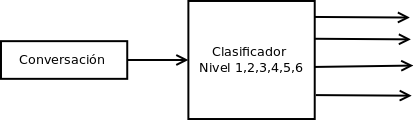
\includegraphics[scale=.5]{images/arquitecturaprotipo4}
\caption{Arquitectura prototipo 4}
\label{fig:arquitecturaNivel4}
\end{center}
\end{figure} 

\subsection{Dise\~no de la red neuronal}
La arquitectura que tendr\'a la red neuronal est\'a presentado en la figura \ref{fig:redNeuronal} donde la capa de entrada represantan los vectores de los niveles descritos anteriormente, la capa oculta est\'a constituida por 7 neuronas y la capa de salida por 4.

\begin{figure}
\begin{center}
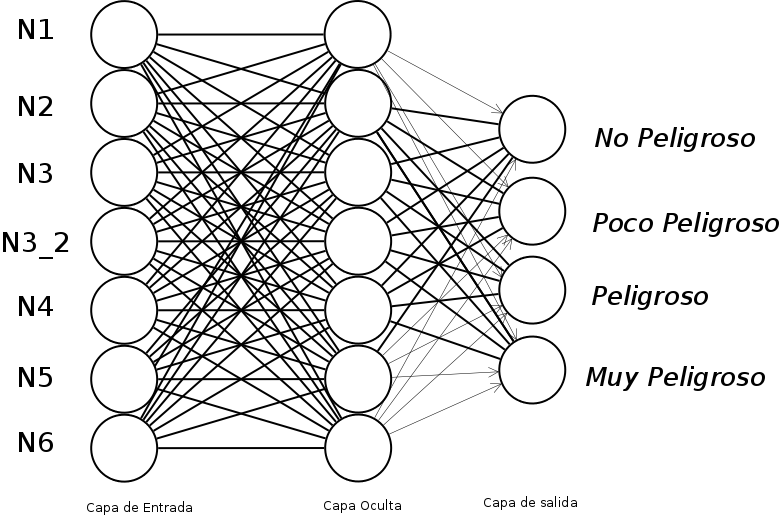
\includegraphics[scale=.5]{images/redneuronal}
\caption{Arquitectura de la Red Neuronal del prototipo 4}
\label{fig:redNeuronal}
\end{center}
\end{figure}

Dicha red fue entrenada con el algorimo de aprendizaje Backpropagation.

\section{Pruebas} 

La figurura \ref{fig:mconfucion} muestra la matriz de confusi\'on donde se muestra una precisi\'on del 98.9\%.

\begin{figure}[h]
\begin{center}
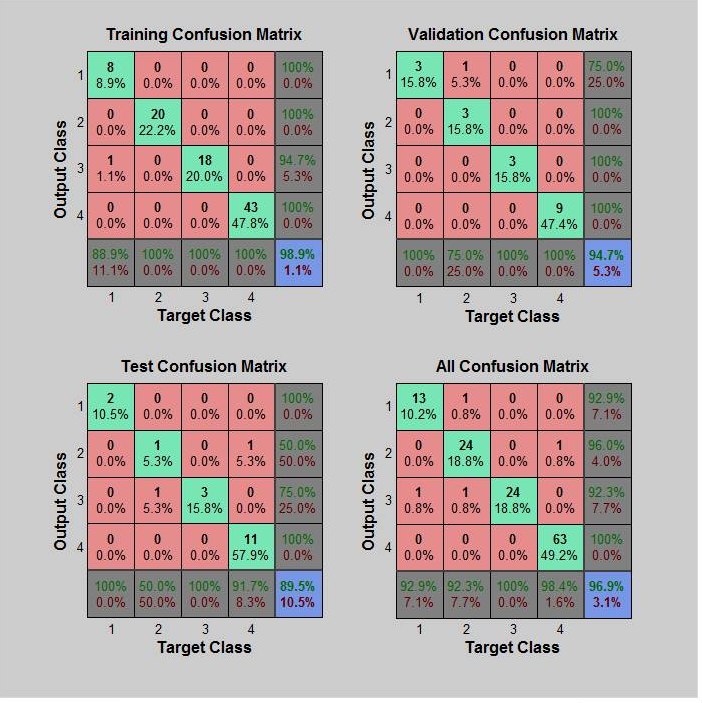
\includegraphics[scale=.5]{images/mcofucion}
\caption{Matriz de confusi\'on del clasificador}
\label{fig:mconfucion}
\end{center}
\end{figure}

